\documentclass[a4paper,12pt]{article}
\setcounter{secnumdepth}{5}
\setcounter{tocdepth}{3}
\usepackage[margin=1in,foot=1in]{geometry}
\usepackage{pgfplots}
\pgfplotsset{compat=1.18}
\input{/usr/share/LaTeX-ToolKit/template.tex}
\begin{document}
\title{微積分 Homework 1}
\author{沈威宇}
\date{\temtoday}
\titledoc
\sct*{1.4 Exercises}
1. (a) $-1$ (b) $3^{-6}$ (c) $x^{-\frac{5}{4}}$ (d) $x^2$ (e) $\frac{b^5}{9}$ (f) $\frac{2x^6}{9y}$

2. (a) $\frac{1}{3}$ (b) $9$ (c) $18x^{12}$ (d) $\frac{x^3}{8}$ (e) $3a^3$ (f) $a^{\frac{1}{6}}b^{-\frac{1}{12}}$

3. (a) $f(x)=b^x$ (b) $\mathbb{R}$ (c) $\{x|x\in\mathbb{R}\land x>0\}$ (d)

(i)
\begin{center}
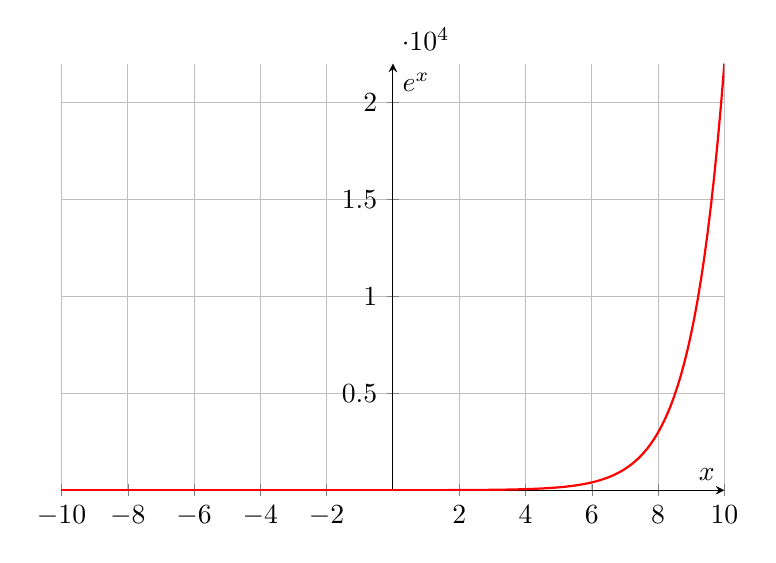
\begin{tikzpicture}
  \begin{axis}[
    axis lines = middle,
    xlabel = $x$,
    ylabel = {$e^x$},
    domain=-10:10,
    samples=200,
    width=10cm, height=7cm,
    grid=both
  ]
    \addplot[red, thick] {exp(x)};
  \end{axis}
\end{tikzpicture}
\end{center}

(ii)
\begin{center}
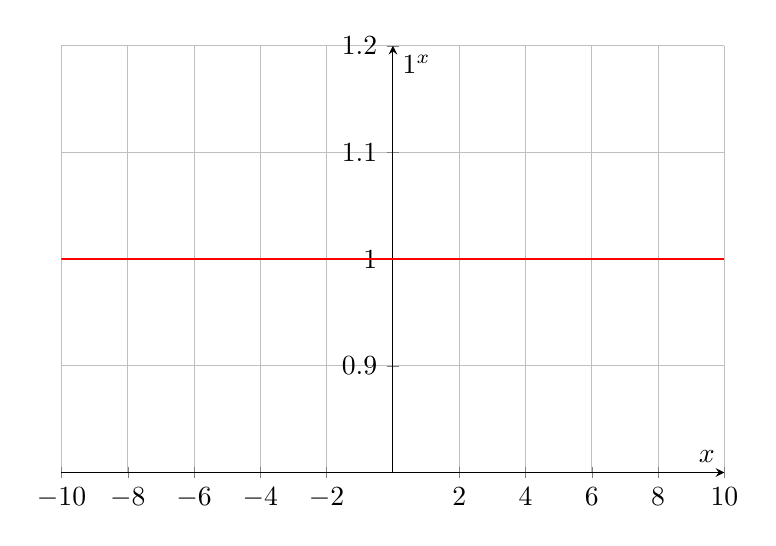
\begin{tikzpicture}
  \begin{axis}[
    axis lines = middle,
    xlabel = $x$,
    ylabel = {$1^x$},
    domain=-10:10,
    samples=200,
    width=10cm, height=7cm,
    grid=both
  ]
    \addplot[red, thick] {1};
  \end{axis}
\end{tikzpicture}
\end{center}

(iii)
\begin{center}
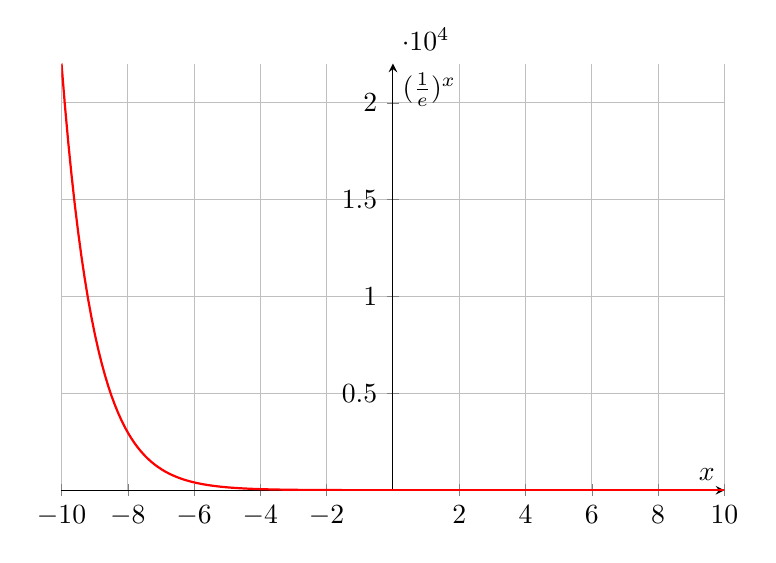
\begin{tikzpicture}
  \begin{axis}[
    axis lines = middle,
    xlabel = $x$,
      ylabel = {$\qty(\frac{1}{e})^x$},
    domain=-10:10,
    samples=200,
    width=10cm, height=7cm,
    grid=both
  ]
    \addplot[red, thick] {exp(-x)};
  \end{axis}
\end{tikzpicture}
\end{center}

4. (a) $\lim_{n\to\infty}\qty(1+\frac{1}{n})^n$ (b) 2.718 (c) $f\colon\mathbb{C}\to\mathbb{C}\setminus\{0\};\;x\mapsto e^x$

5. They are all exponential functions with a base greater than $1$, that is, they lie entirely in the first and second quadrants and are strictly increasing.

6. $y=e^x$ and $y=e^{-x}$ are symmetric about the y-axis; $y=8^x$ and $y=8^{-x}$ are symmetric about the y-axis.

7. $y=3^x$ and $y=\qty(\frac{1}{3})^{-x}$ are symmetric about the y-axis; $y=10^x$ and $y=\qty(\frac{1}{10})^{-x}$ are symmetric about the y-axis.

8. They are all exponential functions with a base less than $1$, that is, they lie entirely in the first and second quadrants and are strictly decreasing.

9.
\begin{center}
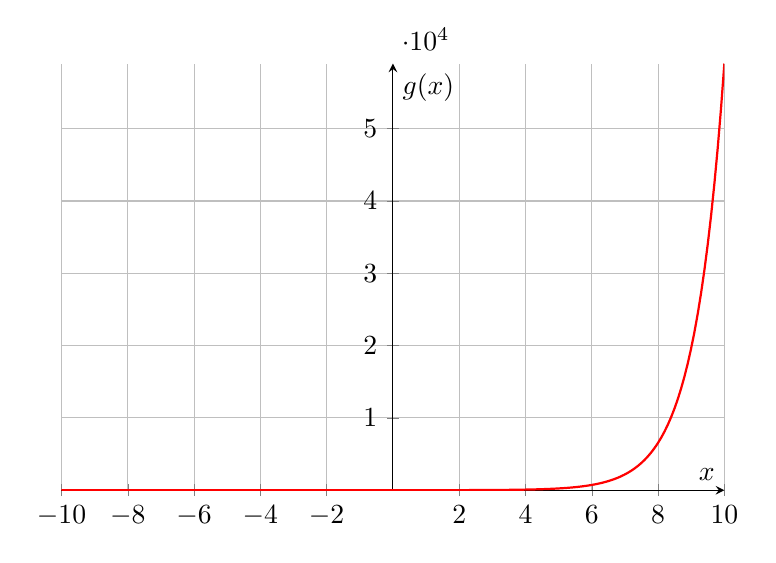
\begin{tikzpicture}
  \begin{axis}[
    axis lines = middle,
    xlabel = $x$,
    ylabel = {$g(x)$},
    domain=-10:10,
    samples=200,
    width=10cm, height=7cm,
    grid=both
  ]
      \addplot[red, thick] {exp(x*ln(3))+1};
  \end{axis}
\end{tikzpicture}
\end{center}

10. 
\begin{center}
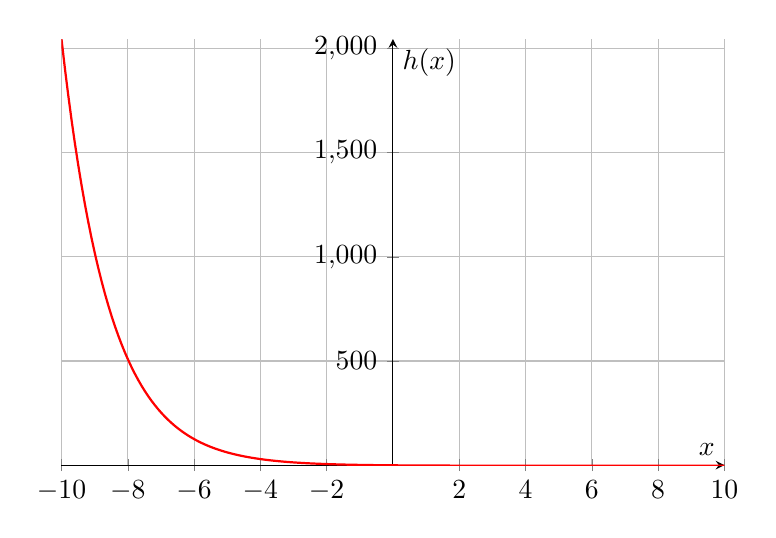
\begin{tikzpicture}
  \begin{axis}[
    axis lines = middle,
    xlabel = $x$,
    ylabel = {$h(x)$},
    domain=-10:10,
    samples=200,
    width=10cm, height=7cm,
    grid=both
  ]
      \addplot[red, thick] {2*exp(x*ln(0.5))-3};
  \end{axis}
\end{tikzpicture}
\end{center}

11.
\begin{center}
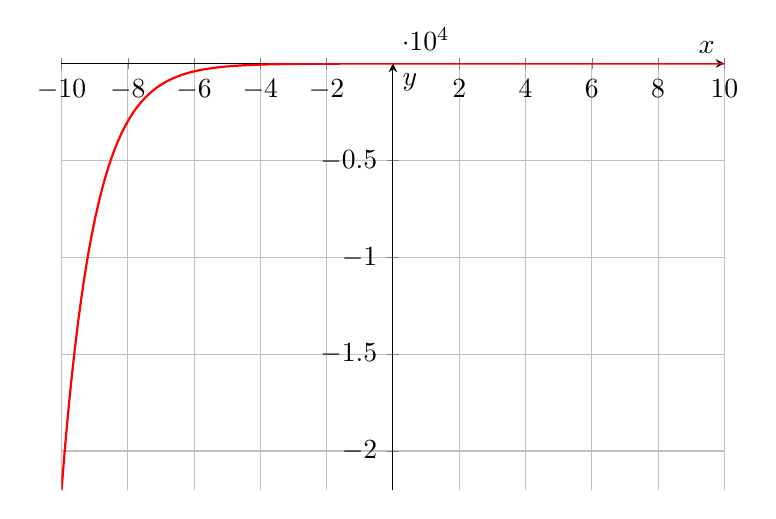
\begin{tikzpicture}
  \begin{axis}[
    axis lines = middle,
    xlabel = $x$,
    ylabel = $y$,
    domain=-10:10,
    samples=200,
    width=10cm, height=7cm,
    grid=both
  ]
      \addplot[red, thick] {-exp(-x)};
  \end{axis}
\end{tikzpicture}
\end{center}

12.
\begin{center}
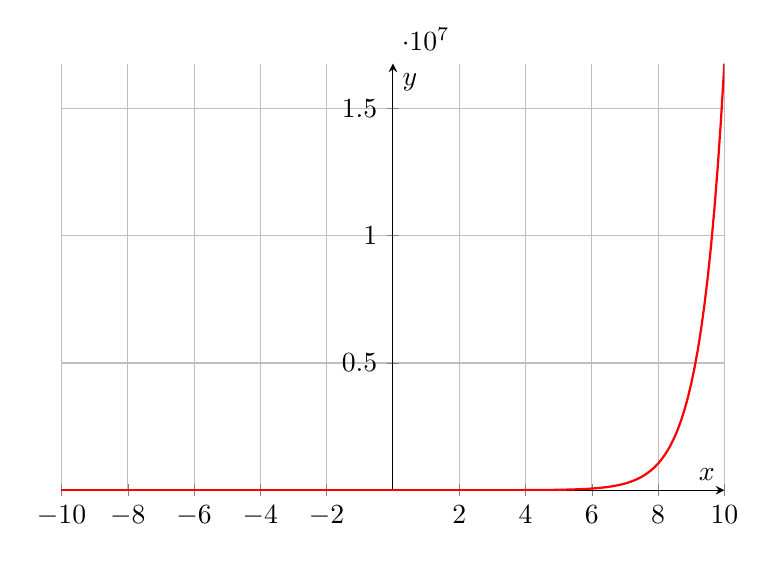
\begin{tikzpicture}
  \begin{axis}[
    axis lines = middle,
    xlabel = $x$,
    ylabel = $y$,
    domain=-10:10,
    samples=200,
    width=10cm, height=7cm,
    grid=both
  ]
      \addplot[red, thick] {exp(ln(4)*(x+2))};
  \end{axis}
\end{tikzpicture}
\end{center}

13.
\begin{center}
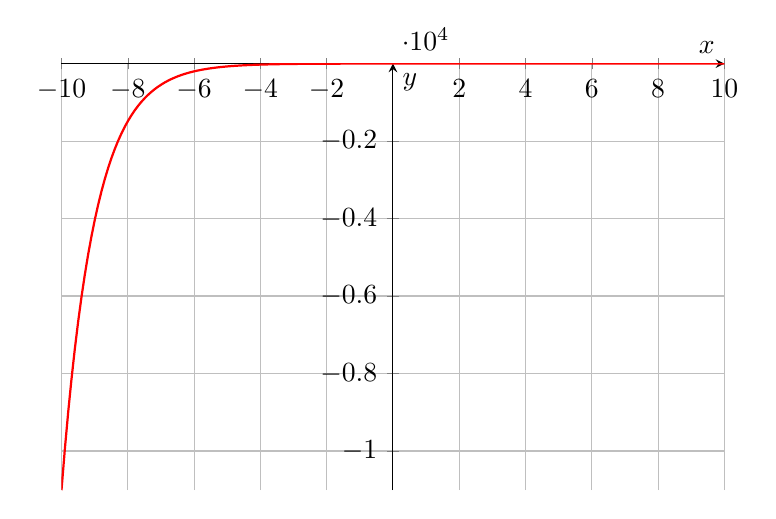
\begin{tikzpicture}
  \begin{axis}[
    axis lines = middle,
    xlabel = $x$,
    ylabel = $y$,
    domain=-10:10,
    samples=200,
    width=10cm, height=7cm,
    grid=both
  ]
      \addplot[red, thick] {1-0.5*exp(-x)};
  \end{axis}
\end{tikzpicture}
\end{center}

14.
\begin{center}
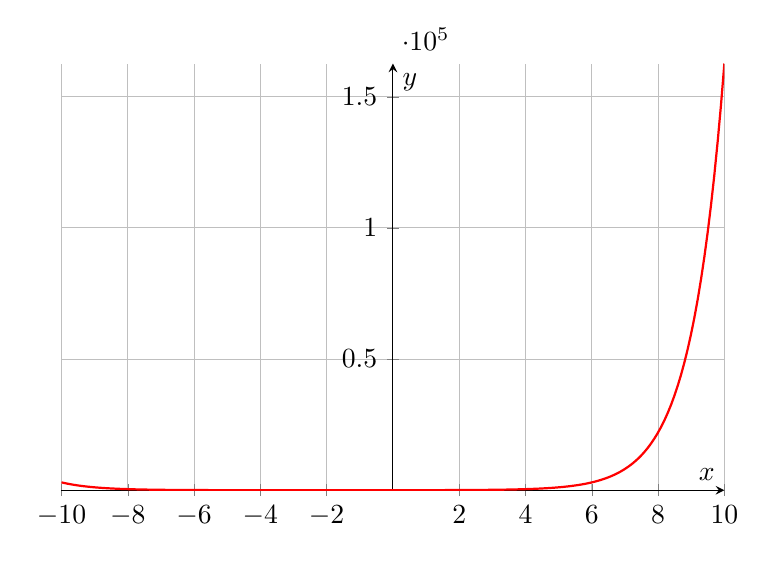
\begin{tikzpicture}
  \begin{axis}[
    axis lines = middle,
    xlabel = $x$,
    ylabel = $y$,
    domain=-10:10,
    samples=200,
    width=10cm, height=7cm,
    grid=both
  ]
      \addplot[red, thick] {exp(abs(x+2))};
  \end{axis}
\end{tikzpicture}
\end{center}

15. (a) $e^x-2$ (b) $e^{x-2}$ (c) $-e^x$ (d) $e^{-x}$ (e) $-e^{-x}$

16. (a) $8-e^x$ (b) $e^{4-x}$

17. (a) $\mathbb{R}\setminus\{-1,1\}$ (b) $\mathbb{R}$

18. (a) $[2,\infty)$ (b) $\mathbb{R}$

19. $f(x)=3\cdot 2^x$

20. $f(x)=2\qty(\frac{2}{3})^x$

21.
\[\frac{f(x+h)-f(x)}{h}=\frac{5^{x+h}-5^x}{h}=5^x\qty(\frac{5^h-1}{h}).\]

22. II. Because:
\[\sum_{n=1}^{30}2^{n-1}=\frac{2^{30}-1}{2-1}=2^{30}-1\approx 10^9\gg 10^6.\]

23. The question statement is incorrect.

24. $(\approx 1.8, \approx 17.1), (5.0, 3125.0)$. $g(x)$.

25. When $x\approx 1.1$.

26. $20.8$.
\begin{center}
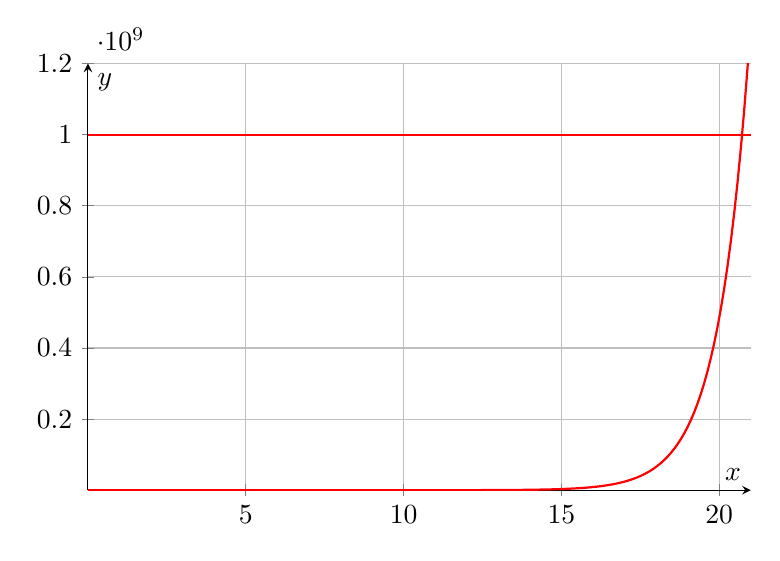
\begin{tikzpicture}
  \begin{axis}[
    axis lines = middle,
    xlabel = $x$,
    ylabel = $y$,
    domain=0:21,
    ymin=0, ymax=1.2e9,
    samples=200,
    width=10cm, height=7cm,
    grid=both
  ]
      \addplot[red, thick] {exp(x)};
      \addplot[red, thick] {1e9};
  \end{axis}
\end{tikzpicture}
\end{center}

\sct*{1.5 Exercises}
1. (a) A function $f$ is a one-to-one function if for any $a\neq b$ in its domain, $f(a)\neq f(b)$. (b) Give both the domain and codomain of the function an arbitary total order such that the equality or inequality of two elements is preserved for any two elements, plot the function on a coordinate plane of them, with domain axis being horizontal and codomain being vertical axis, draw horizontal line for all element in the codomain, if any of the lines intersect with the graph of the function, the function is not one-to-one; otherwise, it is one-to-one.

2. (a) $f^{-1}$ is defined as a function $f^{-1}\colon B\to A$ that maps $f(x)$ to $x$ for any $x\in A$. (b) Convert the original formula to a form such that one side becomes the independent variable and the other side without the independent variable with the axiom of equality, and then replace the independent variable with $f^{-1}$ and $f$ of the independent variable with the new independent variable. (c) Change the label $f$ to the independent variable and the label of the independent variable to $f^{-1}$.

\sct*{2.1 Exercises}
1. (a) $-44.4$, $-38.8$, $-27.8$, $-22.2$, $-16\frac{2}{3}$. (b) $-33.3$ (c) skipped

2. (a) (i) $99$ (ii) $106.3$ (iii) $91.4$. The average number of steps she walks per minute in the time interval.

\sct*{2.2 Exercises}
1. For any $\epsilon>0$, there exists $\delta>0$ such that $0<|x-2|<\delta\implies|f(x)-5|<\epsilon$. Yes, the limit at $x=a$ is independent to the function value at $x=a$.

2. For any $\epsilon>0$, there exists $\delta>0$ such that $0<1-x<\delta\implies|f(x)-3|<\epsilon$; and, for any $\epsilon>0$, there exists $\delta>0$ such that $0<x-1<\delta\implies|f(x)-7|<\epsilon$. No, a limit exists only one both left-side and right-side limit exist and are equal.

3. (a) For any $\epsilon>0$, there exists $\delta>0$ such that $0<|x+3|<\delta\implies f(x)>\epsilon$. (b) For any $\epsilon<0$, there exists $\delta>0$ such that $0<x-4<\delta\implies f(x)<\epsilon$.

4. (a) $3$ (b) $1$ (c) DNE (d) $3$ (e) $4$ (f) DNE

5. (a) $2$ (b) 1 (c) 4 (d) DNE (e) 3

6. (a) $4$ (b) $4$ (c) $4$ (d) DNE (e) $1$ (f) $-1$ (g) DNE (h) $1$ (i) $2$ (j) DNE (k) $3$ (l) DNE

7. (a) $4$ (b) $5$ (c) $2$ (d) $4$

8. (a) $\infty$ (b) $-\infty$ (c) $\infty$ (d) $-\infty$ (e) $x=-3, x=-1, x=2$

\end{document}
